% License:
% CC BY-NC-SA 3.0 (http://creativecommons.org/licenses/by-nc-sa/3.0/)
%----------------------------------------------------------------------------------------
%	PACKAGES AND OTHER DOCUMENT CONFIGURATIONS
%----------------------------------------------------------------------------------------
\documentclass[paper=letter, fontsize=12pt]{scrartcl} % A4 paper and 11pt font size
\usepackage[margin=1in]{geometry}
\usepackage[T1]{fontenc} % Use 8-bit encoding that has 256 glyphs
\usepackage[english]{babel} % English language/hyphenation
\usepackage{sectsty} % Allows customizing section commands
\allsectionsfont{\centering \normalfont\scshape} % Make all sections centered, the default font and small caps
\usepackage{amsmath}
\usepackage{fancyhdr} % Custom headers and footers
\pagestyle{fancyplain} % Makes all pages in the document conform to the custom headers and footers
\fancyhead{} % No page header - if you want one, create it in the same way as the footers below
\fancyfoot[L]{} % Empty left footer
\fancyfoot[C]{\thepage} % Empty center footer
\fancyfoot[R]{} % Page numbering for right footer
\renewcommand{\headrulewidth}{0pt} % Remove header underlines
\renewcommand{\footrulewidth}{0pt} % Remove footer underlines
\setlength{\headheight}{13.6pt} % Customize the height of the header
\usepackage{graphicx}
\usepackage{wrapfig}
\usepackage{hyperref}
\usepackage{setspace}
\usepackage{color}
%\doublespacing

%----------------------------------------------------------------------------------------
%	TITLE SECTION
%----------------------------------------------------------------------------------------

\newcommand{\horrule}[1]{\rule{\linewidth}{#1}} % Create horizontal rule command with 1 argument of height

\title{	
	\normalfont \normalsize 
	\textsc{Working Draft for Hindsight Conference\\APA New York Metro Chapter Diversity Committee\\November 2, 2018} \\ [6pt] % Your university, school and/or department name(s)
	\horrule{1pt} \\[0.5cm] % Thin top horizontal rule
	\huge Measuring the Impacts of Redlining\\% The assignment title
	\horrule{1pt}\\[0.5cm] % Thick bottom horizontal rule
}
\author{Addison Larson} % Your name
\date{\normalsize{\today}} % Today's date or a custom date

\begin{document}
	
	\maketitle % Print the title
	\newpage
	\tableofcontents
	\newcommand{\blankpage}{
		\newpage
		%\thispagestyle{empty}
		\mbox{}
		\newpage
	}
	\listoftables
	\listoffigures
	%\blankpage
	% ----------------------------------
	% START PAPER
	% ----------------------------------
	\section{Introduction}
	Housing policy has historically been a tool for racial discrimination. From the 1930s to the 1950s, the Home Owners' Loan Corporation (HOLC) and the Federal Housing Administration (FHA) used the racial makeup of a neighborhood to determine the risk of a given mortgage applicant \cite{rothstein}. All-white neighborhoods received the best ratings, while neighborhoods with several Black residents received the worst ratings of ``Definitely Declining'' or ``Hazardous'' \cite{richmond}.\par
	This project quantifies the impacts of redlining on today's urban landscape through an analysis of digitized maps of Home Owners' Loan Corporation (HOLC) redlining, data on job accessibility via transit, and 2016 Census estimates for 17 U.S. metropolitan areas. A one-point decrease in HOLC rating correlates with the following modern-day effects: 
	\begin{enumerate}
		\item \textbf{\$62,175 decrease} in median home value, controlling for housing unit size, age, and facilities;
		\item \textbf{13.96\% decrease} in homeownership;
		\item \textbf{2.79\% increase} in rent burden;
		\item \textbf{25,185 additional jobs} accessible via transit;
		\item \textbf{10.87\% increase} in transit-dependent households;
		\item \textbf{\$3,107 decrease} in annual household income, controlling for education levels; and
		\item \textbf{10.66\% increase} in household poverty.
	\end{enumerate}
	Many neighborhoods remain racially segregated along the lines once drawn by HOLC and the FHA. \textbf{In 2016, Black residents were 15.153\% more likely, and white residents 16.806\% less likely, to live in redlined or downgraded census tracts.}
	
	Though the 1968 Fair Housing Act prohibited housing discrimination on the basis of race, the absence of racially discriminatory housing policies has not translated into equity in terms of accessing education or building wealth through higher incomes or homeownership. The results of this project indicate the need for to both be conscious of the disparate racial impacts of urban planning and policy and to actively seek racial equity --- and not merely the absence of discrimination --- through the implementation of housing policy.\par
	
	\section{Problem Statement and Project Objective}
	This study is based on three premises:
	\begin{enumerate}
		\item Cities in the U.S. are racially segregated.
		\item Racially discriminatory housing policies have facilitated segregation in cities.
		\item The location of one's home sets the stage for one's future prospects, including access to a quality education and access to jobs for which one is qualified. These factors affect one's ability to earn an income and accumulate wealth over time.
	\end{enumerate}
	
	\subsection{Racial Segregation in U.S. Cities}
	\textbf{Cities in the U.S. are racially segregated.} The index of dissimilarity is a common measure of spatial segregation. In this case, it measures the percentage of residents that would need to move in order to attain racial parity throughout the metropolitan area. The index value can range from 0 to 1, where 1 indicates complete racial segregation \cite{duncan}. Refer to Table 1: \textit{Indices of Black-White Dissimilarity for 17 U.S. Metro Areas} for a measure of racial segregation in 2016.\par
	
	\begin{table}[h]
		\caption{Indices of Black-White Dissimilarity for 17 U.S. Metro Areas}
		\begin{center}
			\begin{tabular}{||l | c||}
				\hline
				\textbf{Metropolitan Statistical Area} & \textbf{D\textsubscript{I}} \\
				\hline \hline
				Atlanta, GA & 0.560 \\
				\hline
				Baltimore, MD & 0.626 \\
				\hline
				Birmingham, AL & 0.649 \\
				\hline
				Buffalo-Niagara Falls, NY & 0.708 \\
				\hline
				Charlotte-Gastonia-Rock Hill, NC-SC & 0.505 \\
				\hline
				Columbus, OH & 0.600 \\
				\hline
				Indianapolis, IN & 0.627 \\
				\hline
				Kansas City, MO-KS & 0.574 \\
				\hline
				Louisville, KY-IN & 0.568 \\
				\hline
				Minneapolis-St. Paul, MN-WI & 0.542 \\
				\hline
				New Orleans, LA & 0.631 \\
				\hline
				Norfolk-Virginia Beach-Newport News, VA-NC & 0.472 \\
				\hline
				Pittsburgh, PA & 0.657 \\
				\hline
				Portland-Vancouver, OR-WA & 0.488 \\
				\hline
				San Diego, CA & 0.441 \\
				\hline
				St. Louis, MO-IL & 0.709 \\
				\hline
				Tampa-St. Petersburg-Clearwater, FL & 0.511 \\
				\hline
			\end{tabular}
		\end{center}
		Author's calculations from 2016 ACS 5-Year Estimates, Table B02001 \cite{acs16}.
	\end{table}
	
	Several scholars have sought to explain segregation in U.S. cities; three primary hypotheses have emerged from their work.\footnote{For more on this topic, see Blalock, H.M. (1967). \textit{Toward a theory of minority-group relations}. New York: John Wiley \& Sons.} The first is a hypothesis of ``socioeconomic class'': Black residents are typically poorer than white residents and therefore cannot afford to live in wealthy, majority-white neighborhoods. The second is that of ``prejudice'' or ``voluntary segregation'': residents prefer\footnote{There is evidence against this theory in the context of the dissimilarity index. Between 1970 and 1990, the dissimilarity index fell 17\%, coinciding with the elimination of several racially discriminatory barriers to housing after the Fair Housing Act of 1968 \cite{goering2}. If residents preferred to segregrate themselves, the dissimilarity index would not have changed so substantially.} to live among people of the same race and sort themselves into racially homogeneous neighborhoods. The third explanation is ``discrimination'' or ``involuntary segregation'': institutional structures and policies force residents to live in neighborhoods they might not have chosen otherwise, \textit{ceteris paribus}. Galster's review of empirical evidence for these three theories suggests that ``discrimination'' or ``involuntary segregation'' has the most explanatory power \cite{goering}.
	
	\subsection{Housing Policy and Racial Segregation}
	\textbf{Racially discriminatory housing policies have facilitated segregation in cities.} Beginning in 1933 and 1934, repspectively, the Home Owners' Loan Corporation (HOLC) and the Federal Housing Administration (FHA) provided Americans the opportunity to purchase homes through mortgage lending. However, these federally-created programs were racially discriminatory in their administration. Real estate agents employed by the HOLC and the FHA created color-coded maps of U.S. cities, grading neighborhoods along a four-point scale from \textit{A} to \textit{D}. Applications to purchase homes in green neighborhoods --- ``Class A'' --- were nearly guaranteed approval; applications to purchase homes in red neighborhoods --- ``Class D'' --- were almost always denied. ``Class A'' neighborhoods were all-white neighborhoods; ``Class D'' neighborhoods were home to at least some Black residents. The first FHA \textit{Underwriting Manual} of 1935 offered the guidance: ``If a neighborhood is to retain stability it is necessary that properties shall continue to be occupied by the same social and racial classes. A change in social or racial occupancy generally leads to instability and a reduction in values.'' \cite{rothstein} HOLC and FHA lending practices gave birth to the term ``redlining,'' after those neighborhoods downgraded by the agencies \cite{rothstein}.\par
	
	HOLC and FHA lending practices were as biased in their effects as in their administration. First, redlining enforced racial segregation in cities, because it encouraged white residents to purchase homes in all-white neighborhoods and prevented Black residents from moving into these neighborhoods. Second, redlining encouraged a divergence in wealth between Black and white residents. White residents received a generous opportunity to build generational wealth through home equity. Meanwhile, Black residents were systematically discriminated against in the housing market, forced to pay exorbitant prices for substandard rental housing \cite{orfield}, and barred from the chance to buy homes that often serve as a valuable financial investment. Redlining is but one example among a legacy of racially discriminatory housing policies.\par
	
	Redlining can be attributed both to the HOLC and the FHA. For brevity's sake, references in this paper to the neighborhood scoring mechanism associated with redlining will use the term ``HOLC rating.''
	
	\subsection{Home as a Platform for (Dis)Opportunity}
	\textbf{The location of one's home sets the stage for one's future prospects, including access to a quality education and access to jobs for which one is qualified. These factors affect one's ability to earn an income and accumulate wealth over time.} The educational quality of children has lifelong impacts on earnings and educational attainment. Students placed in small classrooms in grades K through 3 had a 1.8\% higher rate of college attendance by age 20 compared to their peers in larger classrooms. \cite{chetty2} In addition, children who moved to low-poverty neighborhoods at a young age had higher rates of college attendance, a 30.8\% increase in annual earnings, and a lifetime income boost of \$302,000. \cite{chetty}.\par
	Employment matters for at least two reasons: it is a means of earning income and a key component of self-worth \cite{blair}. Historically, Black residents have had higher rates of unemployment \cite{wilson}. Some of the explanations in the literature have been spatial in nature, as the opportunities one pursues are partially a function of one's home location. Higher rates of unemployment among Black residents in the city center have been attributed to prohibitive distance to relevant job opportunities, or ``spatial mismatch'' \cite{kain1},  and the decentralization in low-wage and service-sector employment, or ``job sprawl'' \cite{briggs}.\par
	Whether one considers it consequential or coincidental, the Black-white disparity in wealth is stark and well-documented: in 2011, ``white households could draw on \$92,000 to tide them over the rough times, while black families had to stretch a nest egg of \$4,900.'' \cite{goldfield}\par
	
	\subsection{Project Objective}
	Recognizing the role of racial segregation in housing and the effects of home location on education, income, and wealth, this project has two aims: first, to \textbf{quantify the impact of HOLC redlining} on education, work, income, and wealth today; and second, to \textbf{evaluate redlining's disparate and lingering racial effects} between Black and white residents.\par
	
	\section{Hypothesized Relationships}
	\subsection{Hypotheses}
	\begin{enumerate}
		\item \textbf{Access to Education:} Current educational attainment will be lower in downgraded HOLC neighborhoods.
		\item \textbf{Access to Jobs via Transit:} Because downgraded HOLC neighborhoods are typically located close to the city center, more jobs will be accessible via transit.
		\item \textbf{Income and Wealth:} Current incomes, home value, and homeownership will be lower in downgraded HOLC neighborhoods; poverty, unemployment, and rental burdens will be higher.
	\end{enumerate}
	\subsection{Variable Selection and Expectation}
	\begin{enumerate}
		\item \textbf{Access to Education}\\
		\textit{Description:} The percentage of residents who have completed the following: 1) high school diploma or its equivalent; 2) some college; 3) four-year degree; and 4) graduate or professional degrees. Note that educational attainment serves here as a rough proxy for access to quality education services in general. (All measures at the census tract level.)\\
		\textit{Expected Relation to HOLC redlining:} As the HOLC rating decreases:
		\begin{enumerate}
			\item The percentage of residents with a high school diploma or its equivalent will increase;
			\item The percentage of residents with some college will increase;
			\item The percentage of residents with a four-year degree will decrease; and
			\item The percentage of residents with a graduate or professional degree will decrease.
		\end{enumerate}
		
		\item \textbf{Access to Jobs via Transit}\\
		\textit{Description:} The number of jobs accessible within 30 minutes of a census tract using transit. Note that the data says nothing about job sector, pay, or skill requirements. (All measures at the census tract level.)\\
		\textit{Expected Relation to HOLC redlining:} As the HOLC rating decreases, the access to jobs via transit will increase, because redlined neighborhoods, transit service, and jobs are all concentrated in the urban core.
		
		\item \textbf{Income and Wealth}\\
		\textit{Description:} 1) Median household income, with educational attainment as a control factor. 2) The percentage of owner-occupied housing units. 3) Median home value, with housing age, size, and facilities as control factors. 4) Percentage of households below 100\% and 150\% of the Federal Poverty Level (FPL) respectively. 5) Percentage of unemployed residents in the labor force. 6) Median gross rent as a percentage of annual income. (All measures at the census tract level.)\\
		\textit{Expected Relation to HOLC redlining:} As the HOLC rating decreases:
		\begin{enumerate}
			\item Median household income will decrease;
			\item The percentage of owner-occupied housing units will decrease;
			\item Median home value will decrease;
			\item The percentage of households in poverty will increase;
			\item The percentage of unemployed residents will increase; and
			\item Renters will spend a larger percent of their income on rent.
		\end{enumerate}
	\end{enumerate}
	
	\section{Study Area, Data Sources, Methodology, and Analysis}
	\subsection{Study Area}
	Two of the data sources used in this study are limited in their geographic coverage. First, the University of Richmond's ``Mapping Inequality'' project has digitized HOLC redlining maps for 128 cities. Some of the digitized maps must be merged together to better correspond to one MSA (e.g. St. Louis, MO and East St. Louis, IL), resulting in fewer than 128 potential study areas. Second, the University of Minnesota's ``Access Across America'' project has computed job accessibility by transit for 46 of the 50 largest metro areas. Any MSAs with areas present in both the HOLC redlining maps and the job accessibility files are included in the study area (see Figure 1).\par
	\begin{figure}[h]
		\centering
		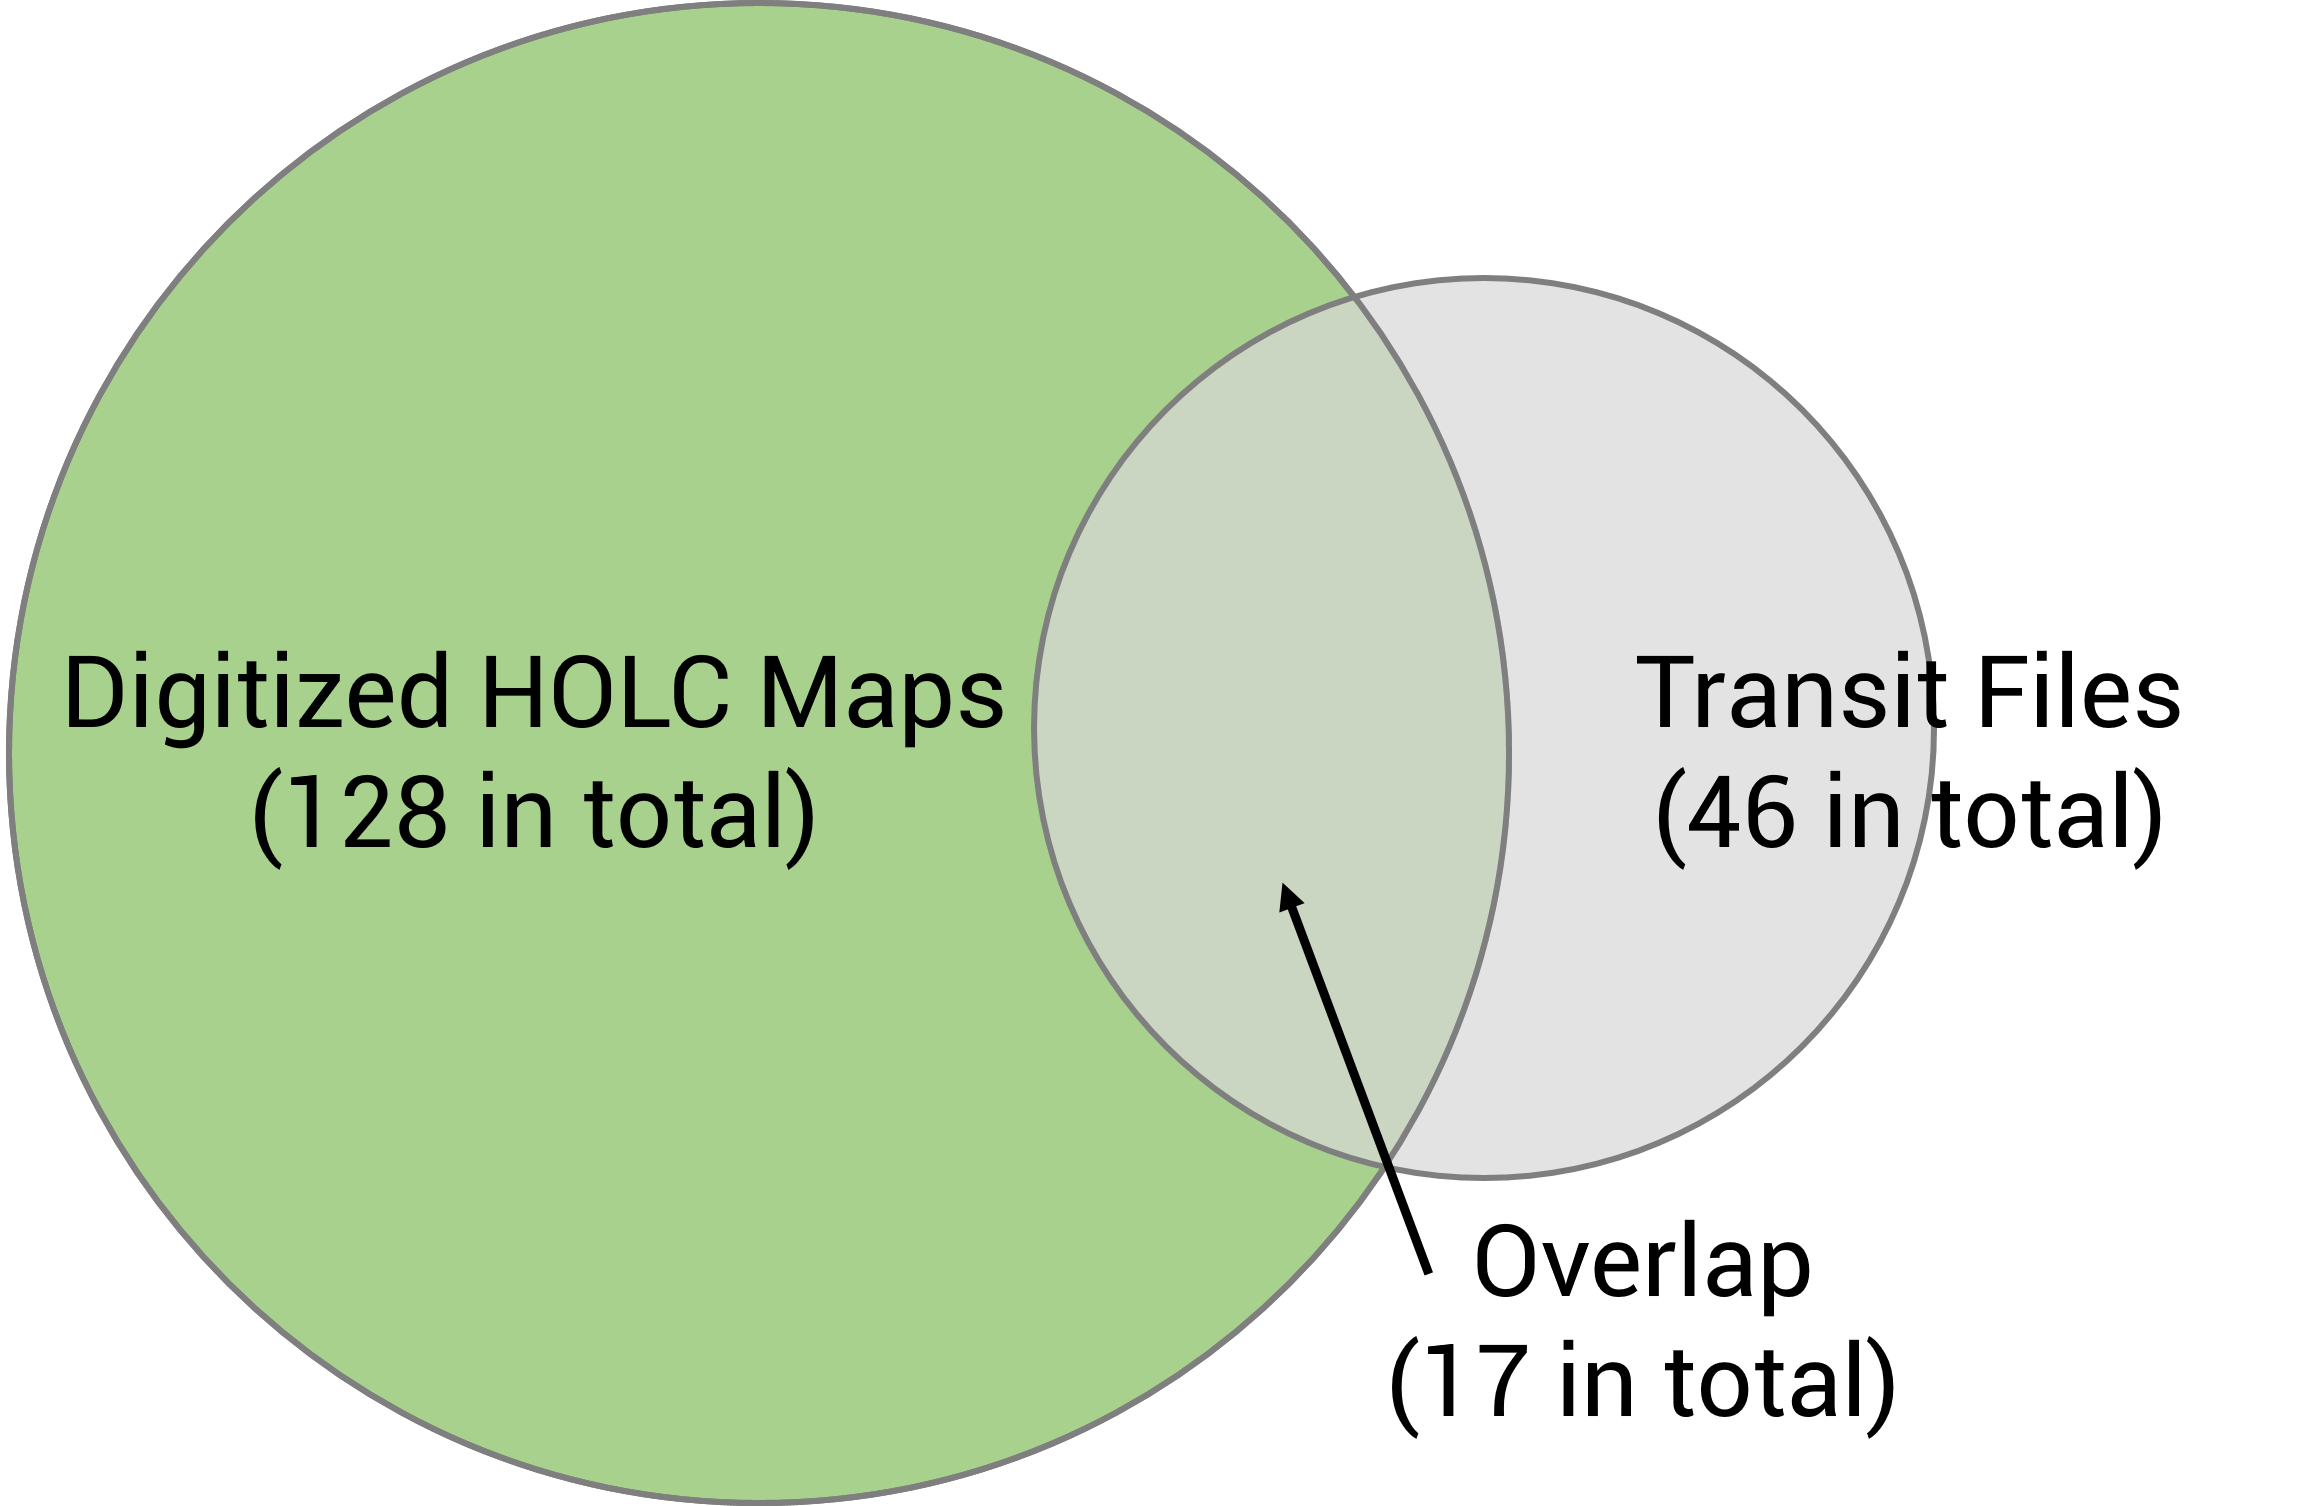
\includegraphics[width = 4.5in]{StudyAreaSelection}\\
		\caption{Overlap of MSAs present in digitized HOLC maps and transit accessibility files}
	\end{figure}
	These MSAs include: Birmingham, AL; San Diego, CA; Tampa-St. Petersburg-Clearwater, FL; Atlanta, GA; St. Louis, MO-IL; Indianapolis, IN; Kansas City, MO-KS; Louisville, KY-IN; New Orleans, LA; Baltimore, MD; Minneapolis-St. Paul, MN; Buffalo-Niagara Falls, NY; Charlotte-Gastonia-Rock Hill, NC-SC; Columbus, OH; Portland-Vancouver, OR-WA; Pittsburgh, PA; and Norfolk-Virginia Beach-Newport News, VA-NC.
	\subsection{Data Sources, Methodology, and Analysis}
	This project utilizes four primary sources of information:
	\begin{enumerate}
		\item \textbf{Shapefiles from the Census Bureau's Topologically Integrated Geographic Encoding and Referencing (TIGER/Line) collection.} \cite{tiger17}\\
		TIGER/Line shapefiles are available for every state at the census tract level. Because some MSAs span state borders, 21 state shapefiles are used, including AL, CA, FL, GA, IL, IN, KS, KY, LA, MD, MN, MO, NC, NY, OH, OR, PA, SC, VA, WA, and WI. These files are subset by \textit{GEOID} to match the spatial extent of MSAs, and census tracts outside MSA boundaries are removed from the files to speed computation.
		\item \textbf{Digitized Shapefiles of Redlining Maps from the University of Richmond's Digital Scholarship Lab.} \cite{richmond} \\
		\textit{American Panorama's} ``Mapping Inequality'' project has digitized HOLC maps from 128 cities and towns. These shapefiles trace the boundaries of HOLC neighborhoods and include the HOLC rating as an attribute. Historic HOLC neighborhood boundaries do not align with present-day census tract boundaries. As an approximation of HOLC rating at the census tract level, each HOLC rating is assigned a numeric value (``Class A'' = 4; ``Class D'' = 1). A union operation is performed in GIS with all census tract shapefiles at the MSA level. The union produces three scenarios, which are handled in statistical software:
		\begin{enumerate}
			\item When a unique \textit{GEOID} is associated with only one HOLC rating, it is given that rating. These cases occur when the HOLC neighborhood encompasses the entire census tract or when the census tract is located on the periphery of the historic HOLC map, thereby overlapping with only one HOLC neighborhood.
			\item When a unique \textit{GEOID} is associated with multiple HOLC ratings, it is assigned the mean of these ratings. Note that this methodology is imperfect and does not account for the area of overlap. One way to account for the area of overlap is to rasterize both the census tract and HOLC rating shapefiles and then to compute the mean HOLC rating by \textit{GEOID}. See \textsection5.3, \textit{Proposed Alterations and Additions}.
			\item When a unique \textit{GEOID} is not associated with any HOLC rating, it is given the value \texttt{NA}. These cases typically occur when the MSA falls outside the periphery of the historic HOLC map or when the MSA is located in the Central Business District.
		\end{enumerate}
		\item \textbf{Job Accessibility Files from the University of Minnesota's \textit{Access Across America: Transit 2014} Study.} \cite{owen} \\
		The \textit{Access Across America} project quantifies the number of jobs that can be accessed within 30 minutes of one's home, as approximated by the census block. However, the spatial unit of this study was the census tract and not the block. It is not suitable to collapse the blocks into tracts and add the number of observations, because jobs will then be counted several times. As an approximation of job accessibility at the census tract level, the job accessibility observations at the block level are collapsed to the tract level, and the mean job accessibility of the constituent block groups is assigned to the tract.
		\item \textbf{Demographic and Commuting Characteristics from the Census Bureau's 2016 American Community Survey (ACS) 5-Year Estimates.} \cite{acs16}\\
		Tables B01001, B06011, B08122, B02001, B03001, B25064, B25077, B25035, B25003, B25041, B25048, B25051, B23025, B15003, B08201, B25071, B11001, C15002A, and C15002B are used in the analysis.
	\end{enumerate}
	While all data is available at the city or MSA level, the primary aim of the study is to identify trends that are not specific to a single city. This requires that all cities be analyzed simultaneously. However, OLS methods are not suitable because an inherent two-class hierarchical (city, nation) structure is present in the data. Variable coefficient, fixed-slope multilevel models are used because they control for within-city correlation.
	
	\clearpage
	
	\begin{table}[h!]
		\caption{Summary of Census Tract Characteristics by HOLC Rating}
		\begin{center}
			\begin{tabular}{|| l | c c c c ||}
				\hline
				Variable & Class A & Class B & Class C & Class D \\
				\hline \hline
				Number of Observations & 5 & 60 & 188 & 140\\
				\hline 
				Avg. Tract Population & 3,680 & 3,222 & 2,974 & 2,490\\
				\hline 
				\multicolumn{5}{|| c ||}{Housing}\\
				\hline 
				Median Home Value, 1000s & \$388.4 & \$250.1 & \$172.7 & \$168.1\\
				\hline 
				Pct. Owner-Occupied Housing Units & 78.65 & 57.77 & 38.51 & 33.30\\
				\hline 
				Median Home Age, Years & 79.0 & 74.2 & 66.6 & 65.0\\
				\hline 
				Median Monthly Rent & \$1097 & \$1008 & \$876 & \$839\\
				\hline 
				Median Gross Rent as \% of Ann. Inc (GRAPI) & 27.36 & 30.06 & 34.54 & 36.81\\
				\hline 
				\multicolumn{5}{|| c ||}{Job Access}\\
				\hline 
				No. Jobs Accessible by Transit & 40,675 & 52,348 & 53,014 & 79,074\\
				\hline 
				Pct. Zero-Car Households & 2.79 & 13.95 & 20.25 & 28.84\\
				\hline 
				Pct. Unemployed in Labor Force & 3.85 & 7.27 & 11.49 & 13.61\\
				\hline 
				\multicolumn{5}{|| c ||}{Income and Poverty Trends}\\
				\hline 
				Annual Median Household Income & \$50,849 & \$34,640 & \$23,236 & \$19,542\\
				\hline 
				Pct. Households Below 150\% FPL & 1.74 & 6.88 & 14.18 & 17.78\\
				\hline 
				Pct. Households Below 100\% FPL & 2.65 & 6.28 & 10.77 & 12.66\\
				\hline 
				Pct. Single-Parent Households & 7.99 & 16.39 & 25.88 & 28.82\\
				\hline 
				\multicolumn{5}{|| c ||}{Education}\\
				\hline 
				Pct. HS Degree or Equivalent & 7.17 & 18.69 & 25.73 & 28.13\\
				\hline 
				Pct. Some College, No Degree & 11.84 & 17.53 & 20.99 & 18.96\\
				\hline 
				Pct. 4-Year College Degree & 38.07 & 26.53 & 18.59 & 12.43\\
				\hline 
				Pct. Grad./Prof. Degree & 36.05 & 21.77 & 11.22 & 8.33\\
				\hline 
				\multicolumn{5}{|| c ||}{Race \& Ethnicity}\\
				\hline 
				Pct. White Residents & 86.69 & 62.24 & 47.04 & 40.71\\
				\hline 
				Pct. Black Residents & 4.59 & 28.47 & 40.55 & 45.07\\
				\hline 
				Pct. Asian Residents & 4.51 & 3.37 & 4.27 & 3.38\\
				\hline 
				Pct. Hispanic Residents & 2.65 & 6.03 & 13.02 & 22.57\\
				\hline 
				Pct. Majority-White Tracts & 100 & 75 & 47 & 29\\
				\hline 
				Pct. Majority-Black Tracts & 0 & 25 & 47 & 61\\
				\hline 
				Pct. Majority-Asian Tracts & 0 & 0 & 1 & 0\\
				\hline 
				Pct. Majority-Hispanic Tracts & 0 & 0 & 4 & 10\\
				\hline 
			\end{tabular}
		\end{center}
		Author's calculations from the following: \textit{(1)} Nelson et al. (2018) \cite{richmond} \textit{(2)} Owen \& Levinson (2014) \cite{owen} \textit{(3)} 2016 ACS 5-Year Estimates, Tables B01001, B06011, B08122, B02001, B03001, B25064, B25077, B25035, B25003, B25041, B25048, B25051, B23025, B15003, B08201, B25071, and B11001 \cite{acs16}. All means are weighted by tract population.
	\end{table}
	
	\begin{table}
		\textbf{HOLC Rating and Home Value.} A one-point decrease in HOLC rating corresponds to a \$62,175 decrease in median home value, controlling for housing unit size, age, and facilities. Interestingly, there is a negative relationship between median home values and housing unit size: census tracts with higher percentages of larger homes are associated with lower home values. This may be because smaller homes are more frequently located in the city center, where housing costs are the highest. Going forward, a more reliable method will use appraisal data to relate home value to HOLC rating and control by housing unit characteristics at the parcel level. See \textsection5.3, \textit{Proposed Alterations and Additions}.
		\caption{Multilevel Model: Home Value, \$1000s}
		\begin{center}
			\begin{tabular}{|| l | c c c ||}
				\hline
				Variable & $\beta$ & SE & \textit{p} \\
				\hline \hline
				Intercept & -172.806 & 486.170 & 0.722 \\
				\hline
				HOLC Score & 62.175 & 7.545 & 0.001*** \\
				\hline
				0 Bedrooms & -3.235 & 1.911 & 0.091* \\
				\hline
				1 Bedroom & -4.339 & 1.404 & 0.002*** \\
				\hline
				2 Bedrooms & -5.768 & 1.332 & 0.001*** \\
				\hline
				3 Bedrooms & -7.101 & 1.374 & 0.001*** \\
				\hline
				4 Bedrooms & -2.787 & 1.869 & 0.137 \\
				\hline
				Age of Home & 0.474 & 0.404 & 0.241 \\
				\hline
				Complete Plumbing Facilities & 9.436 & 4.549 & 0.039** \\
				\hline
				Complete Kitchen Facilities & -2.021 & 0.540 & 0.001*** \\
				\hline
				Birmingham, AL & 94.098 & 91.656 & 0.305 \\
				\hline
				San Diego, CA & 209.557 & 86.443 & 0.016** \\
				\hline
				Tampa, FL & 15.954 & 91.818 & 0.862 \\
				\hline
				Atlanta, GA & 154.585 & 98.984 & 0.119 \\
				\hline
				St. Louis, MO & -75.060 & 86.462 & 0.386 \\
				\hline
				Indianapolis, IN & -18.228 & 85.483 & 0.831 \\
				\hline
				Kansas City, MO & -50.450 & 86.560 & 0.560 \\
				\hline
				Louisville, KY & -64.334 & 88.052 & 0.465 \\
				\hline
				New Orleans, LA & 132.570 & 86.993 & 0.128 \\
				\hline
				Baltimore, MD & 14.845 & 86.299 & 0.864 \\
				\hline
				Minneapolis, MN & -22.681 & 85.886 & 0.792 \\
				\hline
				Buffalo, NY & -70.195 & 90.658 & 0.439 \\
				\hline
				Charlotte, NC & 114.962 & 95.065 & 0.227 \\
				\hline
				Columbus, OH & -12.475 & 89.531 & 0.889 \\
				\hline
				Portland, OR & 81.021 & 128.403 & 0.528 \\
				\hline
				Pittsburgh, PA & -48.048 & 86.774 & 0.580 \\
				\hline
				Norfolk, VA & NA & NA & NA \\
				\hline
			\end{tabular}
		\end{center}
		\textit{SE} = 84.05 on 361 degrees of freedom. \textit{Adj. R\textsuperscript{2}} = 0.587. \textit{F} = 22.96 on 25 and 361 degrees of freedom, \textit{p} = 0.001. Norfolk, VA Boolean variable is removed because of multicollinearity.\\
		Author's calculations from the following: \textit{(1)} Nelson et al. (2018) \cite{richmond} \textit{(2)} 2016 ACS 5-Year Estimates, Tables B25035, B25041, B25048, B25051, and B25077 \cite{acs16}.
	\end{table}
	
	\begin{table}
		\textbf{HOLC Rating and Home Ownership.} A one-point decrease in HOLC rating corresponds to a 13.962\% decrease in home ownership.
		\caption{Multilevel Model: Percentage Home Ownership}
		\begin{center}
			\begin{tabular}{|| l | c c c ||}
				\hline
				Variable & $\beta$ & SE & \textit{p} \\
				\hline \hline
				Intercept & 16.829 & 16.790 & 0.317\\
				\hline 
				HOLC Score & 13.962 & 1.323 & 0.001***\\
				\hline 
				Birmingham, AL & -6.927 & 17.788 & 0.697\\
				\hline 
				San Diego, CA & -16.784 & 16.719 & 0.316\\ 
				\hline 
				Tampa, FL & 9.923 & 17.867 & 0.579\\
				\hline 
				Atlanta, GA & -14.675 & 19.063 & 0.442\\
				\hline 
				St. Louis, MO & -7.313 & 16.640 & 0.661\\
				\hline 
				Indianapolis, IN & 5.645 & 16.630 & 0.734\\
				\hline 
				Kansas City, MO & 6.406 & 16.731 & 0.702\\
				\hline 
				Louisville, KY & 2.007 & 17.043 & 0.906\\
				\hline 
				New Orleans, LA & 2.548 & 16.792 & 0.879\\
				\hline 
				Baltimore, MD & -1.682 & 16.634 & 0.920\\
				\hline 
				Minneapolis, MN & -4.847 & 16.627 & 0.771\\
				\hline 
				Buffalo, NY & -11.866 & 17.597 & 0.501\\
				\hline 
				Charlotte, NC & -20.407 & 18.412 & 0.268\\
				\hline 
				Columbus, OH & -20.846 & 17.136 & 0.225\\
				\hline 
				Portland, OR & -27.509 & 23.289 & 0.238\\
				\hline 
				Pittsburgh, PA & -5.618 & 16.718 & 0.737\\
				\hline 
				Norfolk, VA & NA & NA & NA\\
				\hline 
			\end{tabular}
		\end{center}
		\textit{SE} = 16.46 on 374 degrees of freedom. \textit{Adj. R\textsuperscript{2}} = 0.301. \textit{F} = 10.9 on 17 and 374 degrees of freedom, \textit{p} = 0.001. Norfolk, VA Boolean variable is removed because of multicollinearity.\\
		Author's calculations from the following: \textit{(1)} Nelson et al. (2018) \cite{richmond} \textit{(2)} 2016 ACS 5-Year Estimates, Table B25003 \cite{acs16}.
	\end{table}
	
	\begin{table}
		\textbf{HOLC Rating and Rent Burdens.} A one-point decrease in HOLC rating corresponds to a 2.794\% increase in median census tract income spent on rent (GRAPI, or ``Gross Rent as a Percentage of Annual Income''). While median rents are lower in census tracts with lower HOLC ratings, incomes are also lower in these tracts, leading to higher rental burdens. This may partially explain the negative relationship between GRAPI and median rent: census tracts with high median rents often have residents with high incomes who can afford the rent. However, it is worth noting that all census tracts in the study area had GRAPI values on the cusp of or exceeding the U.S. Department of Housing and Urban Development (HUD) standard of affordability. HUD defines a housing unit as affordable if it costs less than 30\% of a resident's income, or GRAPI below 30\%. (See Table 2, \textit{Summary of Census Tract Characteristics by HOLC Rating}.)
		\caption{Multilevel Model: Median Gross Rent as a Percentage of Annual Income}
		\begin{center}
			\begin{tabular}{|| l | c c c ||}
				\hline
				Variable & $\beta$ & SE & \textit{p} \\
				\hline \hline
				Intercept & 	53.444	 & 	7.986	 & 	0.001***	\\ 
				\hline 
				HOLC Rating & 	-2.794	 & 	0.682	 & 	0.001***	\\ 
				\hline 
				Median Rent (\$100s) & 	-0.790	 & 	0.214	 & 	0.001***	\\ 
				\hline 
				Birmingham, AL & 	-8.728	 & 	8.323	 & 	0.295	\\ 
				\hline 
				San Diego, CA & 	-3.187	 & 	7.808	 & 	0.683	\\ 
				\hline 
				Tampa, FL & 	-1.643	 & 	8.337	 & 	0.844	\\ 
				\hline 
				Atlanta, GA & 	-11.817	 & 	8.898	 & 	0.185	\\ 
				\hline 
				St. Louis, MO & 	-3.554	 & 	7.784	 & 	0.648	\\ 
				\hline 
				Indianapolis, IN & 	-6.377	 & 	7.765	 & 	0.412	\\ 
				\hline 
				Kansas City, MO & 	-7.294	 & 	7.820	 & 	0.352	\\ 
				\hline 
				Louisville, KY & 	-7.561	 & 	7.965	 & 	0.343	\\ 
				\hline 
				New Orleans, LA & 	-5.347	 & 	7.838	 & 	0.496	\\ 
				\hline 
				Baltimore, MD & 	-6.439	 & 	7.761	 & 	0.407	\\ 
				\hline 
				Minneapolis, MN & 	-8.115	 & 	7.758	 & 	0.296	\\ 
				\hline 
				Buffalo, NY & 	-11.675	 & 	8.233	 & 	0.157	\\ 
				\hline 
				Charlotte, NC & 	-9.865	 & 	8.591	 & 	0.252	\\ 
				\hline 
				Columbus, OH & 	0.826	 & 	8.011	 & 	0.918	\\ 
				\hline 
				Portland, OR & 	-2.887	 & 	10.873	 & 	0.791	\\ 
				\hline 
				Pittsburgh, PA & 	-9.434	 & 	7.814	 & 	0.228	\\ 
				\hline 
				Norfolk, VA & 	NA	 & 	NA	 & 	NA	\\ 
				\hline 
			\end{tabular}
		\end{center}
		\textit{SE} = 7.68 on 371 degrees of freedom. \textit{Adj. R\textsuperscript{2}} = 0.167. \textit{F} = 5.33 on 18 and 371 degrees of freedom, \textit{p} = 0.001. Norfolk, VA Boolean variable is removed because of multicollinearity.\\
		Author's calculations from the following: \textit{(1)} Nelson et al. (2018) \cite{richmond} \textit{(2)} 2016 ACS 5-Year Estimates, Tables B25064 and B25071 \cite{acs16}.
	\end{table}
	
	\begin{table}
		\textbf{HOLC Rating and Job Accessibility.} A one-point decrease in HOLC rating corresponds to 25,185 additional jobs accessible within a 30-minute commute via transit. This is likely because most of the low-rated HOLC neighborhoods were located in the urban core, where we also observe higher job and transit density.
		\caption{Multilevel Model: Number of Jobs Accessible via Transit, 1000s}
		\begin{center}
			\begin{tabular}{|| l | c c c ||}
				\hline
				Variable & $\beta$ & SE & \textit{p}\\
				\hline \hline
				Intercept & 65.063 & 41.055 & 0.114\\ 
				\hline 
				HOLC Rating & -25.185 & 3.229 & 0.001***\\ 
				\hline 
				Birmingham, AL & 9.755 & 43.499 & 0.823\\ 
				\hline 
				San Diego, CA & 26.425 & 40.884 & 0.518\\ 
				\hline 
				Tampa, FL & 12.812 & 43.692 & 0.770\\ 
				\hline 
				Atlanta, GA & 86.118 & 46.616 & 0.065*\\ 
				\hline 
				St. Louis, MO & 26.354 & 40.693 & 0.518\\ 
				\hline 
				Indianapolis, IN & 5.317 & 40.667 & 0.896\\ 
				\hline 
				Kansas City, MO & 21.970 & 40.915 & 0.592\\ 
				\hline 
				Louisville, KY & 17.992 & 41.678 & 0.666\\ 
				\hline 
				New Orleans, LA & 10.574 & 41.064 & 0.797\\ 
				\hline 
				Baltimore, MD & 95.251 & 40.674 & 0.020**\\ 
				\hline 
				Minneapolis, MN & 109.502 & 40.659 & 0.007***\\ 
				\hline 
				Buffalo, NY & 46.962 & 43.033 & 0.276\\ 
				\hline 
				Charlotte, NC & 92.656 & 45.025 & 0.040**\\ 
				\hline 
				Columbus, OH & 59.141 & 41.904 & 0.159\\ 
				\hline 
				Portland, OR & 149.996 & 56.950 & 0.009***\\ 
				\hline 
				Pittsburgh, PA & 76.705 & 40.882 & 0.061*\\ 
				\hline 
				Norfolk, VA & NA & NA & NA\\ 
				\hline 
			\end{tabular}
		\end{center}
		\textit{SE} = 40.25 on 375 degrees of freedom. \textit{Adj. R\textsuperscript{2}} = 0.502. \textit{F} = 24.22 on 17 and 375 degrees of freedom, \textit{p} = 0.001. Norfolk, VA Boolean variable is removed because of multicollinearity.\\
		Author's calculations from the following: \textit{(1)} Nelson et al. (2018) \cite{richmond} \textit{(2)} Owen \& Levinson (2014) \cite{owen}.
	\end{table}
	
	\begin{table}
		\textbf{HOLC Rating and Zero-Car Households.} A one-point decrease in HOLC rating corresponds to a 10.869\% increase in zero-car households. One way to read this is that these households have better transit access, making it unnecessary to own a car. Another way to read this is these residents are transit-dependent and would prefer a car if they could afford one. The correlation between income and zero-car households for the study area (-0.631), and Table 2, \textit{Summary of Census Tract Characteristics by HOLC Rating}, both demonstrate that zero-car households are often poorer households.
		\caption{Multilevel Model: Percentage Zero-Car Households}
		\begin{center}
			\begin{tabular}{|| l | c c c ||}
				\hline
				Intercept & 32.628 & 11.661 & 0.005***\\ 
				\hline 
				HOLC Rating & -10.869 & 0.919 & 0.001***\\ 
				\hline 
				Birmingham, AL & 7.746 & 12.354 & 0.531\\ 
				\hline 
				San Diego, CA & -0.551 & 11.611 & 0.962\\ 
				\hline 
				Tampa, FL & 6.001 & 12.409 & 0.629\\ 
				\hline 
				Atlanta, GA & 17.195 & 13.239 & 0.195\\ 
				\hline 
				St. Louis, MO & 22.151 & 11.557 & 0.056*\\ 
				\hline 
				Indianapolis, IN & 3.959 & 11.549 & 0.732\\ 
				\hline 
				Kansas City, MO & 6.970 & 11.620 & 0.549\\ 
				\hline 
				Louisville, KY & 9.383 & 11.837 & 0.428\\ 
				\hline 
				New Orleans, LA & 7.178 & 11.662 & 0.539\\ 
				\hline 
				Baltimore, MD & 27.875 & 11.553 & 0.016**\\ 
				\hline 
				Minneapolis, MN & 11.929 & 11.547 & 0.302\\ 
				\hline 
				Buffalo, NY & 17.558 & 12.221 & 0.152\\ 
				\hline 
				Charlotte, NC & 3.423 & 12.787 & 0.789\\ 
				\hline 
				Columbus, OH & 10.786 & 11.901 & 0.365\\ 
				\hline 
				Portland, OR & 41.854 & 16.174 & 0.010***\\ 
				\hline 
				Pittsburgh, PA & 19.499 & 11.611 & 0.094*\\ 
				\hline 
				Norfolk, VA & NA & NA & NA\\ 
				\hline
			\end{tabular}
		\end{center}
		\textit{SE} = 11.43 on 374 degrees of freedom. \textit{Adj. R\textsuperscript{2}} = 0.489. \textit{F} = 22.97 on 17 and 374 degrees of freedom, \textit{p} = 0.001. Norfolk, VA Boolean variable is removed because of multicollinearity.\\
		Author's calculations from the following: \textit{(1)} Nelson et al. (2018) \cite{richmond} \textit{(2)} 2016 ACS 5-Year Estimates, Table B08201 \cite{acs16}.
	\end{table}
	
	\begin{table}
		\textbf{HOLC Rating and Unemployment.} There is no statistically significant relationship between HOLC rating and unemployment when controlling for education levels. A one-percent increase in residents with a high school degree corresponds to a 0.15\% increase in unemployment; A one-percent increase in residents with a four-year degree corresponds to a 0.25\% decrease in unemployment.
		\caption{Multilevel Model: Percentage Unemployed Individuals in the Labor Force}
		\begin{center}
			\begin{tabular}{|| l | c c c ||}
				\hline
				Variable & $\beta$ & SE & \textit{p}\\
				\hline \hline
				(Intercept) & 8.957 & 5.924 & 0.131\\
				\hline 
				quantScore & -0.656 & 0.463 & 0.158\\
				\hline 
				High School Diploma or Equivalent & 0.153 & 0.054 & 0.005***\\
				\hline 
				Some College & 0.031 & 0.052 & 0.552\\
				\hline 
				Four-Year Degree & -0.253 & 0.046 & 0.001***\\
				\hline 
				Graduate or Professional Degree & -0.060 & 0.052 & 0.251\\
				\hline 
				Birmingham, AL & 4.201 & 5.433 & 0.439\\
				\hline 
				San Diego, CA & 3.091 & 5.174 & 0.551\\
				\hline 
				Tampa, FL & 9.151 & 5.482 & 0.096*\\
				\hline 
				Atlanta, GA & 6.781 & 5.837 & 0.246\\
				\hline 
				St. Louis, MO & 7.965 & 5.095 & 0.119\\
				\hline 
				Indianapolis, IN & 5.263 & 5.095 & 0.302\\
				\hline 
				Kansas City, MO & 3.705 & 5.123 & 0.471\\
				\hline 
				Louisville, KY & 3.932 & 5.214 & 0.451\\
				\hline 
				New Orleans, LA & 5.106 & 5.156 & 0.323\\
				\hline 
				Baltimore, MD & 5.482 & 5.102 & 0.283\\
				\hline 
				Minneapolis, MN & 4.990 & 5.120 & 0.330\\
				\hline 
				Buffalo, NY & 1.819 & 5.419 & 0.737\\
				\hline 
				Charlotte, NC & 9.263 & 5.645 & 0.102\\
				\hline 
				Columbus, OH & 5.336 & 5.247 & 0.310\\
				\hline 
				Portland, OR & 13.431 & 7.120 & 0.060*\\
				\hline 
				Pittsburgh, PA & 5.493 & 5.129 & 0.285\\
				\hline 
				Norfolk, VA & NA & NA & NA\\
				\hline 
			\end{tabular}
		\end{center}
		\textit{SE} = 5.003 on 370 degrees of freedom. \textit{Adj. R\textsuperscript{2}} = 0.588. \textit{F} = 27.51 on 21 and 370 degrees of freedom, \textit{p} = 0.001. Norfolk, VA Boolean variable is removed because of multicollinearity.\\
		Author's calculations from the following: \textit{(1)} Nelson et al. (2018) \cite{richmond} \textit{(2)} 2016 ACS 5-Year Estimates, Tables B15003 and B23025 \cite{acs16}.
	\end{table}
	
	\begin{table}
		\textbf{HOLC Rating and Income.} A one-point decrease in HOLC rating corresponds to a \$3,107 decrease in annual median household income, controlling for education levels. While the education coefficients appear small, they make a big difference in income: for example, if a census tract has 10\% more residents with four-year degrees, that tract is expected to have a \$4,420 increase in annual median household income. This table, and Table 8, \textit{Multilevel Model: Percentage Unemployed Individuals in the Labor Force}, indicate a possibility that higher education can boost incomes and reduce unemployment beyond any residual effects of HOLC rating.
		\caption{Multilevel Model: Annual Median Household Income, \$1000s}
		\begin{center}
			\begin{tabular}{|| l | c c c ||}
				\hline
				Variable & $\beta$ & SE & \textit{p}\\
				\hline \hline
				Intercept & 5.843 & 6.809 & 0.391\\ 
				\hline 
				HOLC Rating & 3.107 & 0.532 & 0.001***\\ 
				\hline 
				High School Diploma or Equivalent & 0.130 & 0.063 & 0.039**\\ 
				\hline 
				Some College &0.081 & 0.059 & 0.174\\ 
				\hline 
				Four-Year Degree &0.442 & 0.052 & 0.001***\\ 
				\hline 
				Graduate or Professional Degree &0.423 & 0.060 & 0.001***\\ 
				\hline 
				Birmingham, AL & -8.156 & 6.247 & 0.193\\ 
				\hline 
				San Diego, CA & -1.987 & 5.950 & 0.739\\ 
				\hline 
				Tampa, FL & -5.009 & 6.304 & 0.427\\ 
				\hline 
				Atlanta, GA & -11.799 & 6.712 & 0.080*\\ 
				\hline 
				St. Louis, MO & -7.597 & 5.859 & 0.196\\ 
				\hline 
				Indianapolis, IN & -4.665 & 5.859 & 0.426\\ 
				\hline 
				Kansas City, MO & -4.769 & 5.899 & 0.419\\ 
				\hline 
				Louisville, KY & -6.618 & 5.996 & 0.270\\ 
				\hline 
				New Orleans, LA & -4.219 & 5.929 & 0.477\\ 
				\hline 
				Baltimore, MD & -4.887 & 5.867 & 0.405\\ 
				\hline 
				Minneapolis, MN & -6.210 & 5.888 & 0.292\\ 
				\hline 
				Buffalo, NY & -8.037 & 6.230 & 0.198\\ 
				\hline 
				Charlotte, NC & -1.343 & 6.491 & 0.836\\ 
				\hline 
				Columbus, OH & -16.189 & 6.033 & 0.008**\\ 
				\hline 
				Portland, OR & -23.340 & 8.188 & 0.005**\\ 
				\hline 
				Pittsburgh, PA & -8.306 & 5.898 & 0.160\\ 
				\hline 
				Norfolk, VA & NA & NA & NA\\ 
				\hline 
			\end{tabular}
		\end{center}
		\textit{SE} = 5.754 on 371 degrees of freedom. \textit{Adj. R\textsuperscript{2}} = 0.741. \textit{F} = 54.58 on 21 and 371 degrees of freedom, \textit{p} = 0.001. Norfolk, VA Boolean variable is removed because of multicollinearity. DEGREES.\\
		Author's calculations from the following: \textit{(1)} Nelson et al. (2018) \cite{richmond} \textit{(2)} 2016 ACS 5-Year Estimates, Tables B15003 and B06001 \cite{acs16}.
	\end{table}
	
	\begin{table}
		\textbf{HOLC Rating and Poverty.} A one-point decrease in HOLC rating corresponds to a 10.659\% increase in households in poverty. Here, poverty is defined as households making less than 150\% of the Federal Poverty Level, or an annual household income below \$36,450 for a family of four in 2016.
		\caption{Multilevel Model: Percentage Households Below 150\% FPL}
		\begin{center}
			\begin{tabular}{|| l | c c c ||}
				\hline
				Variable & $\beta$ & SE & \textit{p}\\
				\hline \hline
				Intercept & 41.370 & 12.329 & 0.001***\\ 
				\hline 
				HOLC Rating & -10.659 & 0.971 & 0.001***\\ 
				\hline 
				Birmingham, AL & 9.146 & 13.062 & 0.484\\ 
				\hline 
				San Diego, CA & 3.814 & 12.277 & 0.756\\ 
				\hline 
				Tampa, FL & 2.880 & 13.120 & 0.826\\ 
				\hline 
				Atlanta, GA & -4.891 & 13.999 & 0.727\\ 
				\hline 
				St. Louis, MO & 9.839 & 12.22 & 0.421\\ 
				\hline 
				Indianapolis, IN & 4.492 & 12.212 & 0.713\\ 
				\hline 
				Kansas City, MO & 6.814 & 12.286 & 0.579\\ 
				\hline 
				Louisville, KY & 6.798 & 12.515 & 0.587\\ 
				\hline 
				New Orleans, LA & -2.250 & 12.331 & 0.855\\ 
				\hline 
				Baltimore, MD & -3.269 & 12.215 & 0.789\\ 
				\hline 
				Minneapolis, MN & 6.650 & 12.209 & 0.586\\ 
				\hline 
				Buffalo, NY & 8.259 & 12.922 & 0.523\\ 
				\hline 
				Charlotte, NC & 9.159 & 13.521 & 0.499\\ 
				\hline 
				Columbus, OH & 21.443 & 12.583 & 0.090*\\ 
				\hline 
				Portland, OR & 17.923 & 17.101 & 0.295\\ 
				\hline 
				Pittsburgh, PA & 2.726 & 12.276 & 0.824\\ 
				\hline 
				Norfolk, VA & NA & NA & NA\\ 
				\hline
			\end{tabular}
		\end{center}
		\textit{SE} = 12.09 on 374 degrees of freedom. \textit{Adj. R\textsuperscript{2}} = 0.275. \textit{F} = 9.742 on 17 and 374 degrees of freedom, \textit{p} = 0.001. Norfolk, VA Boolean variable is removed because of multicollinearity.\\
		Author's calculations from the following: \textit{(1)} Nelson et al. (2018) \cite{richmond} \textit{(2)} 2016 ACS 5-Year Estimates, Table B15003 \cite{acs16}.
	\end{table}
	
	\begin{table}
		\textbf{HOLC Rating and Black Residents.} A one-point decrease in HOLC rating corresponds to a 15.153\% increase in the percentage of Black residents at the census tract level.
		\caption{Multilevel Model: Percentage Black Residents}
		\begin{center}
			\begin{tabular}{|| l | c c c ||}
				\hline
				Variable & $\beta$ & SE & \textit{p}\\
				\hline \hline
				Intercept & 56.889 & 29.401 & 0.054*\\ 
				\hline 
				HOLC Rating & -15.153 & 2.313 & 0.001***\\ 
				\hline 
				Birmingham, AL & 39.635 & 31.151 & 0.204\\ 
				\hline 
				San Diego, CA & -19.943 & 29.278 & 0.496\\ 
				\hline 
				Tampa, FL & 28.447 & 31.289 & 0.364\\ 
				\hline 
				Atlanta, GA & 21.870 & 33.383 & 0.513\\ 
				\hline 
				St. Louis, MO & 47.433 & 29.141 & 0.104\\ 
				\hline 
				Indianapolis, IN & 16.762 & 29.122 & 0.565\\ 
				\hline 
				Kansas City, MO & 15.074 & 29.300 & 0.607\\ 
				\hline 
				Louisville, KY & 17.361 & 29.847 & 0.561\\ 
				\hline 
				New Orleans, LA & 17.895 & 29.407 & 0.543\\ 
				\hline 
				Baltimore, MD & 42.800 & 29.128 & 0.143\\ 
				\hline 
				Minneapolis, MN & 1.187 & 29.117 & 0.968\\ 
				\hline 
				Buffalo, NY & 3.093 & 30.817 & 0.920\\ 
				\hline 
				Charlotte, NC & 12.750 & 32.244 & 0.693\\ 
				\hline 
				Columbus, OH & 16.690 & 30.009 & 0.578\\ 
				\hline 
				Portland, OR & -22.307 & 40.783 & 0.585\\ 
				\hline 
				Pittsburgh, PA & 17.037 & 29.277 & 0.561\\ 
				\hline 
				Norfolk, VA & NA & NA & NA\\ 
				\hline
			\end{tabular}
		\end{center}
		\textit{SE} = 28.83 on 375 degrees of freedom. \textit{Adj. R\textsuperscript{2}} = 0.352. \textit{F} = 13.5 on 17 and 375 degrees of freedom, \textit{p} = 0.001. Norfolk, VA Boolean variable is removed because of multicollinearity.\\
		Author's calculations from the following: \textit{(1)} Nelson et al. (2018) \cite{richmond} \textit{(2)} 2016 ACS 5-Year Estimates, Table B02001 \cite{acs16}.
	\end{table}
	
	\begin{table}
		\textbf{HOLC Rating and White Residents.} On the contrary, a one-point decrease in HOLC rating corresponds to a 16.806\% decrease in the percentage of white residents at the census tract level. This table and the prior table (Table 11, \textit{Multilevel Model: Percentage Black Residents}) indicate that HOLC policies may relate to the persistence of racial segregation in U.S. neighborhoods.
		\caption{Multilevel Model: Percentage White Residents}
		\begin{center}
			\begin{tabular}{|| l | c c c ||}
				\hline
				Variable & $\beta$ & SE & \textit{p}\\
				\hline \hline
				Intercept & 26.399 & 28.136 & 0.349\\ 
				\hline 
				HOLC Rating & 16.806 & 2.213 & 0.001***\\ 
				\hline 
				Birmingham, AL & -27.670 & 29.811 & 0.354\\ 
				\hline 
				San Diego, CA & 7.354 & 28.019 & 0.793\\ 
				\hline 
				Tampa, FL & -19.937 & 29.943 & 0.506\\ 
				\hline 
				Atlanta, GA & -13.836 & 31.948 & 0.665\\ 
				\hline 
				St. Louis, MO & -40.524 & 27.888 & 0.147\\ 
				\hline 
				Indianapolis, IN & -10.391 & 27.870 & 0.709\\ 
				\hline 
				Kansas City, MO & -13.872 & 28.040 & 0.621\\ 
				\hline 
				Louisville, KY & -8.516 & 28.563 & 0.766\\ 
				\hline 
				New Orleans, LA & -8.538 & 28.143 & 0.762\\ 
				\hline 
				Baltimore, MD & -34.355 & 27.875 & 0.219\\ 
				\hline 
				Minneapolis, MN & -7.382 & 27.865 & 0.791\\ 
				\hline 
				Buffalo, NY & -10.496 & 29.492 & 0.722\\ 
				\hline 
				Charlotte, NC & -12.704 & 30.857 & 0.681\\ 
				\hline 
				Columbus, OH & -12.093 & 28.719 & 0.674\\ 
				\hline 
				Portland, OR & 9.904 & 39.03 & 0.800\\ 
				\hline 
				Pittsburgh, PA & -12.822 & 28.018 & 0.647\\ 
				\hline 
				Norfolk, VA & NA & NA & NA\\  
				\hline
			\end{tabular}
		\end{center}
		\textit{SE} = 27.59 on 375 degrees of freedom. \textit{Adj. R\textsuperscript{2}} = 0.272. \textit{F} = 9.618 on 17 and 375 degrees of freedom, \textit{p} = 0.001. Norfolk, VA Boolean variable is removed because of multicollinearity.\\
		Author's calculations from the following: \textit{(1)} Nelson et al. (2018) \cite{richmond} \textit{(2)} 2016 ACS 5-Year Estimates, Table B02001 \cite{acs16}.
	\end{table}
	
	\section{Results and Interpretation}
	\subsection{Lessons Learned}
	\textbf{Hypotheses and Results.} For the most part, expectations and results align relatively closely. Table 13, \textit{Hypotheses and Results}, lists the expectations correlating with a decrease in HOLC rating and the evidence from multilevel models.
	\begin{table}[h!]
		\caption{Hypotheses and Results}
		\begin{center}
			\begin{tabular}{|| l |  c c ||}
				\hline
				Variable & Expectation & Result \\
				\hline \hline
				\multicolumn{3}{|| c ||}{Educational Attainment}\\
				\hline
				Pct. HS Degree or Equivalent & Positive & Positive \\ 
				\hline
				Pct. Some College, No Degree & Positive & Positive \\ 
				\hline 
				Pct. 4-Year College Degree & Negative & Negative \\ 
				\hline 
				Pct. Grad./Prof. Degree & Negative & Negative \\ 
				\hline 
				\multicolumn{3}{|| c ||}{Access to Jobs via Transit}\\
				\hline
				No. Jobs Accessible by Transit & Positive & Positive \\ 
				\hline
				\multicolumn{3}{|| c ||}{Income and Wealth}\\
				\hline
				Annual Median Household Income & Negative & Negative \\ 
				\hline
				Pct. Owner-Occupied Housing Units & Negative & Negative \\ 
				\hline
				Median Home Value & Negative & Negative \\ 
				\hline
				Pct. Households below 150\% FPL & Positive & Positive \\ 
				\hline
				Pct. Unemployed in Labor Force & Positive & No Relationship \\ 
				\hline
				Median Gross Rent as \% of Ann. Inc & Positive & Positive \\ 
				\hline
			\end{tabular}
		\end{center}
	\end{table}
	
	\begin{table}[h!]
		This is population-weighted mean education levels. We can see a stark divergence. So there's really an uphill climb here. When you look at things in the aggregate, it doesn't look so good. However, what can we do on the smaller level?
		\caption{Mean Education Levels by Race and HOLC Rating}
		\begin{center}
			\begin{tabular}{|| l | c c c | c c c ||}
				\hline
				& \multicolumn{3}{c | }{Pct. Black Residents} & \multicolumn{3}{c ||}{Pct. White Residents} \\
				& High School & Some & College & High School & Some & College \\
				& Diploma & College & Diploma & Diploma & College & Diploma \\
				\hline \hline
				Class A & 18.875 & 36.479 & 37.205 & 6.381 & 16.455 & 75.668 \\
				\hline
				Class B & 34.596 & 29.147 & 17.344 & 12.134 & 21.415 & 62.350 \\
				\hline
				Class C & 34.474 & 32.801 & 12.580 & 19.504 & 24.781 & 45.126 \\
				\hline
				Class D & 34.552 & 29.007 & 11.195 & 23.163 & 21.901 & 33.798 \\
				\hline
			\end{tabular}
		\end{center}
		Author's calculations from 2016 ACS 5-Year Estimates, Tables C15002A and C15002B \cite{acs16}. All means are weighted by the total number of observations.
	\end{table}
	
	\subsection{Policy Implications}
	\textbf{Lessons from the Fair Housing Act of 1968.} FIRST, what values and principles did the Fair Housing Act ensconce? However, the iteration of the Fair Housing Act passed by the Senate notoriously conferred no ``teeth'' in enforcement to its administering agency, the U.S. Department of Housing and Urban Development. \par
	
	LOCAL ENFORCEMENT rolf pendall BLACK METROPOLIS IN 21ST CEN john a powell
	
	
	
	\subsection{Proposed Alterations and Additions}
	\textbf{Disregard transit accessibility files to expand the potential study area.} This study rests on the cusp of statistical invalidity; while it has a decent total sample size (\textit{n} = 395 census tracts), some individual MSAs have a paltry number of observations. A more robust study would encompass as many MSAs as possible but only keep those with a relatively large number of observations after spatial overlay with HOLC files. A larger within-MSA sample size would enable the use of more robust statistical techniques such as a random effects multilevel model.\par
	\textbf{Use raster methods to overlay HOLC shapefiles with census tract shapefiles.} When multiple HOLC neighborhoods intersect with a single census tract, the current overlay method, discussed in \textsection3.2, simply takes the mean of the HOLC ratings and assigns this value to the tract. This method assumes an equal contribution of each HOLC rating when it is plausible that a census tract could share 90\% of its area with a HOLC neighborhood in ``Class B'' and only 10\% of its area with a HOLC neighborhood in ``Class A.'' Rasterizing both spatial layers and computing the zonal mean, where the zone is the census tract, would account for the percentage areal contribution of each HOLC rating to the census tract. \par
	\textbf{Control for housing amenities and compute a spatial overlay with HOLC shapefiles at the parcel level.} Another way to circumvent the problem of spatial overlay mentioned above is to disregard census units altogether. County appraisal shapefiles contain rich information about the amenities and condition of every housing unit at the parcel level. Using appraisal data would confer two benefits: 1) Controlling for more variables and analyzing appraised values at the parcel level would enable a more reliable reading of the influence of HOLC rating than is possible in this project; and 2) With only a small percentage of exceptions, housing parcels will definitively lie within or outside of a HOLC neighborhood.
	
	%\blankpage
	%\newpage
	%\section{Figures}
	%\begin{figure}[p]
	%	\centering
	%	\includegraphics[width=8.5in, angle=270]{DalRentLowSESTest}\\
	%	\caption{Clusters of above-median percentages of rental units available assuming a rental budget 30\% of \$15,000 annual gross income. ACS 5-Year Estimates, Tables DP04 and B25064.}
	%\end{figure}
	%\clearpage
	
	
	--------------------------------------------------------------------------------------
	%	BIBLIOGRAPHY
	%----------------------------------------------------------------------------------------
	\clearpage
	
	
	\medskip
	
	\begin{thebibliography}{9}
		\bibitem{blair}
		Blair, J.P., \& Fichtenbaum, R.H. (1992). Changing black employment patterns. In Galster, G.C., \& Hill, E.W. (Eds.), \textit{The metropolis in black and white: Place, power, and polarization}. New Brunswick, NJ: Center for Urban Policy Research.
		\bibitem{briggs}
		Briggs, X., Popkin, S.J., \& Goering, J.M. (2010). \textit{Moving to opportunity: The story of an American experiment to fight ghetto poverty}. New York: Oxford University Press.
		\bibitem{bullard}
		Bullard, R.D. (2007). \textit{The Black metropolis in the twenty-first century: Race, power, and politics of place}. Lanham, MD: Rowman \& Littlefield.
		\bibitem{chetty}
		Chetty, R., Hendren, N., \& Katz, L. (2015). \textit{The effects of exposure to better neighborhoods on children: New evidence from the Moving to Opportunity experiment} (NBER Working Paper 21156). Retrieved from \href{http://www.equality-of-opportunity.org/images/mto_paper.pdf}{http://www.equality-of-opportunity.org/images/mto\_paper.pdf}
		\bibitem{chetty2}
		Chetty, R., Friedman, J.N., Hilger, N., Saez, E., Schanzenbach, D.W., \& Yagan, D. (2011). How does your kindergarten classroom affect your earnings? Evidence from Project STAR. \textit{Quarterly Journal of Economics, 126}(4), 1593-1660.
		\bibitem{duncan}
		Duncan, O.D., \& Duncan, B. (1955). A methodological analysis of segregation indexes. \textit{American Sociological Review, 20}(2): 210-217.
		\bibitem{galster}
		Galster, G.C., \& Hill, E.W. (1992). \textit{The Metropolis in black and white: Place, power, and polarization}. New Brunswick, N.J.: Center for Urban Policy Research.
		\bibitem{goering}
		Galster, G.C. (1986). More than skin deep: The effect of housing discrimination on the extent and pattern of racial segregation in the United States. In Goering, J.M. (Ed.), \textit{Housing desegregation and federal policy} (119-168). Chapel Hill: University of North Carolina Press.
		\bibitem{glaeser}
		Glaeser, E.L., Kahn, M.E., \& Rappaport, J. (2008). Why do the poor live in cities? The role of public transportation. \textit{Journal of Urban Economics, 63}(1): 1-24.
		\bibitem{goering2}
		Goering, J.M. (2007). An overview of key issues in the field of fair housing research. In Goering, J.M. (Ed.), \textit{Fragile rights within cities: Government, housing, and fairness} (21-40). Lanham, MD: Rowman \& Littlefield.
		\bibitem{goldfield}
		Goldfield, D. (2017). \textit{The gifted generation: When government was good}. New York: Bloomsbury.
		\bibitem{kain1}
		Kain, J.F. (1968). Housing segregation, Negro employment, and metropolitan decentralization. \textit{Quarterly Journal of Economics, 82}(2): 175-197.
		\bibitem{kingsley}
		Kingsley, G.T., \& Turner, M.A. (1993). \textit{Housing Markets and residential mobility}. Washington DC: Urban Institute Press.
		\bibitem{richmond}
		Nelson, R.K., Winling, L., Marciano, R., Connolly, N., Madron, J., Ayers, N., \ldots Williams, R. (2018). ``Mapping inequality: Redlining in New Deal America.'' In Nelson, R.K., \& Ayers, E.L. (Eds.), \textit{American panorama: An atlas of United States history}. Retrieved from \href{https://dsl.richmond.edu/panorama/redlining}{https://dsl.richmond.edu/panorama/redlining}
		\bibitem{orfield}
		Orfield, G. (1986). The movement for housing integration: Rationale and the nature of the challenge. In Goering, J.M. (Ed.), \textit{Housing desegregation and federal policy} (18-30). Chapell Hill: University of North Carolina Press.
		\bibitem{owen}
		Owen, A., \& Levinson, D.M. (2014). \textit{Access across America: Transit 2014 data.} [Data file]. Available from \href{http://dx.doi.org/10.13020/D6MW2Q}{http://dx.doi.org/10.13020/D6MW2Q}
		\bibitem{rothstein}
		Rothstein, R. (2017). \textit{The color of law: A forgotten history of how our government segregated America}. New York: Liveright Publishing.
		\bibitem{silverman}
		Silverman, R.M., \& Patterson, K.L. (2012). \textit{Fair and affordable housing in the U.S.: Trends, outcomes, future directions}. Boston: Brill.
		\bibitem{squires}
		Squires, G.D., \& Kubrin, C.E. (2006). \textit{Privileged places: Race, residence, and the structure of opportunity}. Boulder, CO: Lynne Rienner Publishers.
		%\bibitem{stiglitz}
		%Stiglitz, J.E. (2016). \textit{Rewriting the rules of the American economy: An agenda for growth and shared prosperity}. New York: W.W. Norton.
		\bibitem{acs16}
		United States Census Bureau. (2016). \textit{American Community Survey 5-Year Estimates.} [Data file]. Available from \href{https://factfinder.census.gov/faces/nav/jsf/pages/searchresults.xhtml?refresh=t}{https://factfinder.census.gov/faces/nav/jsf/pages/searchresults.xhtml?refresh=t}
		\bibitem{tiger17}
		United States Census Bureau. (2017). \textit{TIGER/Line Shapefiles.} [Data file]. Available from \href{https://www.census.gov/geo/maps-data/data/tiger-line.html}{https://www.census.gov/geo/maps-data/data/tiger-line.html}
		\bibitem{wilson}
		Wilson, W.J. (1987). \textit{The truly disadvantaged: The inner city, the underclass, and public policy.} Chicago: University of Chicago Press.
	\end{thebibliography}
	
	
\end{document}